%% =======================================================
%% Actividad 21: Modelos de clasificación
%%
%% Compilar desde actividades/: ./compilar.sh act21
%% Las figuras de img/ se generan con: python act21.py
%% =======================================================

%% ---- CONFIGURACIÓN ------------------------

\documentclass[11pt,letterpaper]{article}

\usepackage[indice]{tecnm}
\usepackage[T1]{fontenc}
\usepackage{amsmath}
\usepackage{xcolor}
\usepackage[most]{tcolorbox} % Carga tcolorbox con soporte para listings y saltos de página
\tcbuselibrary{listings, skins, breakable}
\setlength{\emergencystretch}{3em} % Evita líneas desbordadas por palabras en \texttt

% Paleta de colores (estilo GitHub Light / VS Code)
\definecolor{codebg}{HTML}{F8F9FA}       % Fondo del código
\definecolor{codehead}{HTML}{E9ECEF}     % Fondo de la barra de título
\definecolor{codeborder}{HTML}{CED4DA}   % Borde de la tarjeta
\definecolor{codetitle}{HTML}{212529}    % Texto del título
\definecolor{codekw}{HTML}{0550AE}       % Palabras clave (import, def, for...)
\definecolor{codefunc}{HTML}{8250DF}     % Funciones y métodos (describe, groupby...)
\definecolor{codestr}{HTML}{0A3069}      % Strings
\definecolor{codecomm}{HTML}{6E7781}     % Comentarios
\definecolor{codenum}{HTML}{8C959F}      % Números de línea
\definecolor{codeid}{HTML}{24292F}       % Texto general

% Configuración base de listings
\lstdefinestyle{pythonestilo}{
  language=Python,
  basicstyle=\ttfamily\footnotesize\color{codeid},
  keywordstyle=\color{codekw}\bfseries,
  keywordstyle=[2]\color{codefunc}, % Estilo secundario para métodos de datos
  stringstyle=\color{teal!80!black},
  commentstyle=\color{codecomm}\itshape,
  morekeywords={as, True, False, None, with, yield, lambda},
  morekeywords=[2]{load_breast_cancer, LogisticRegression, StandardScaler, StratifiedKFold, LeaveOneOut, cross_val_predict, train_test_split, confusion_matrix, roc_auc_score, make_pipeline, fit, predict, predict_proba, print, len, sum, max, DataFrame, Series, value_counts, reindex, mean, std, var, randint, normal, seed, cumsum, poisson, binom, pmf, norm, fit, kde, bincount, linspace, train_test_split, make_blobs, GaussianNB, chisquare, pdf, cdf, hist, bar, plot, axhline, axvline, fill_between, subplots, figure, concat, nunique, load_iris, diff, sort, unique},
  numbers=left,
  numberstyle=\tiny\ttfamily\color{codenum},
  stepnumber=1,
  numbersep=10pt,
  showstringspaces=false,
  morestring=[b]{"""},
  tabsize=4,
  breaklines=true,
  breakatwhitespace=true,
  columns=flexible,
  keepspaces=true,
  literate=
    {á}{{\'a}}1 {é}{{\'e}}1 {í}{{\'i}}1 {ó}{{\'o}}1 {ú}{{\'u}}1
    {Á}{{\'A}}1 {É}{{\'E}}1 {Í}{{\'I}}1 {Ó}{{\'O}}1 {Ú}{{\'U}}1
    {ñ}{{\~n}}1 {Ñ}{{\~N}}1 {¿}{{?`}}1 {¡}{{!`}}1 {°}{{$^\circ$}}1
}

% Definición del entorno personalizado \begin{codigo}{Título}{etiqueta}
% \newtcblisting[auto counter, number within=section]{codigo}[2][]{
\newtcblisting[auto counter]{codigo}[2][]{
  listing only,
  breakable,                    % Permite que el bloque se divida si pasa de página
  enhanced,
  colback=codebg,
  colframe=codeborder,
  colbacktitle=codehead,
  coltitle=codetitle,
  fonttitle=\bfseries\small\sffamily,
  boxrule=0.6pt,
  arc=4pt,                      % Bordes redondeados
  left=20pt,                    % Espacio izquierdo para los números de línea
  right=8pt,
  top=6pt,
  bottom=6pt,
  toptitle=4pt,
  bottomtitle=4pt,
  before skip=12pt,
  after skip=12pt,
  listing options={style=pythonestilo},
  title={Código \thetcbcounter: #2},
  #1
}

% Paleta para salida de consola (estilo terminal limpia)
\definecolor{termbg}{HTML}{212529}      % Fondo oscuro tipo terminal
\definecolor{termhead}{HTML}{343A40}    % Barra superior
\definecolor{termtext}{HTML}{F8F9FA}    % Texto claro de alta legibilidad
\definecolor{termborder}{HTML}{495057}  % Borde

% Entorno \begin{consola}[label=out:iris]{Título}
\newtcblisting[auto counter]{consola}[2][]{
  listing only,
  breakable,
  colback=termbg,
  colframe=termborder,
  colbacktitle=termhead,
  coltitle=termtext,
  colupper=termtext,
  fonttitle=\bfseries\small\sffamily,
  boxrule=0.6pt,
  arc=4pt,
  left=8pt,
  right=8pt,
  top=6pt,
  bottom=6pt,
  toptitle=4pt,
  bottomtitle=4pt,
  before skip=12pt,
  after skip=12pt,
  listing options={
    basicstyle=\ttfamily\scriptsize\color{termtext}, % \scriptsize evita que las tablas de Pandas se partan de línea
    breaklines=true,
    columns=fixed,        % Mantiene alineadas las columnas de Pandas
    keepspaces=true,
    showstringspaces=false,
    literate=
      {á}{{\'a}}1 {é}{{\'e}}1 {í}{{\'i}}1 {ó}{{\'o}}1 {ú}{{\'u}}1
      {Á}{{\'A}}1 {É}{{\'E}}1 {Í}{{\'I}}1 {Ó}{{\'O}}1 {Ú}{{\'U}}1
      {ñ}{{\~n}}1 {Ñ}{{\~N}}1 {°}{{$^\circ$}}1
  },
  title={Salida \thetcbcounter: #2},
  #1
}

%% ---- DATOS DE LA MATERIA ------------------------

\materia{Modelos Estadísticos para el Aprendizaje \\ Automático y Ciencia de Datos}
\actividad{Tema 3.3 Validación Estadística de Modelos de Aprendizaje Automático \\ Actividad 21 - Modelos de clasificación}

\profesor{Dr. José Ismael Ojeda Campaña}
%\fecha{15 de octubre de 2026}    % opcional; por defecto es la fecha de hoy

\begin{document}
\portada
\indicegeneral

%% ---- CONTENIDO ---------------------------------

\section{Introducción}

Antes de que un clasificador opere en un entorno real hace falta una estimación confiable de su efectividad, y esa estimación depende de dos decisiones: con qué métricas se mide y cómo se parten los datos entre entrenamiento y prueba \parencite{tecnm2026_tema33}. La métrica adecuada depende de la naturaleza del problema, y el método de partición depende de la cantidad de datos disponibles: con pocos datos se recurre a alguna validación cruzada y con datos suficientes basta una partición hold-out \parencite{tecnm2026_tema33}.

En esta actividad se elige un conjunto de datos de un repositorio público, el diagnóstico de cáncer de mama de Wisconsin, y se construye un clasificador evaluado con los tres métodos de partición del tema: hold-out, validación cruzada de 10 particiones y leave-one-out. Se compara la estabilidad de cada método según el tamaño del conjunto, se reportan las métricas de efectividad y se justifica cuál es la más adecuada para este problema. El script genera automáticamente las tablas y un resumen del análisis.

\section{Marco conceptual}

\subsection{Matriz de confusión y métricas}

La efectividad de un clasificador se valida comúnmente con la matriz de confusión, una matriz cuadrada cuyas entradas cuentan las predicciones correctas e incorrectas. En el caso binario sus entradas son verdaderos positivos (VP), falsos positivos (FP), falsos negativos (FN) y verdaderos negativos (VN). La clase positiva es la de mayor interés: en un problema de enfermos y sanos, es menos costoso asignar la clase enfermo a una persona sana (falso positivo) que sano a una persona enferma (falso negativo) \parencite{tecnm2026_tema33}. Las métricas del tema se calculan con esas cuatro cantidades \parencite{tecnm2026_tema33}:
\begin{align*}
\text{Exactitud} &= \frac{VP + VN}{VP + VN + FP + FN}, &
\text{Precisión} &= \frac{VP}{VP + FP}, &
\text{Sensibilidad} &= \frac{VP}{VP + FN},\\
\text{Especificidad} &= \frac{VN}{VN + FP}, &
F_1 &= \frac{2 \cdot \text{Precisión} \cdot \text{Sensibilidad}}{\text{Precisión} + \text{Sensibilidad}}.
\end{align*}
La exactitud es el porcentaje global de aciertos, pero no es adecuada con conjuntos desbalanceados porque su resultado se sesga hacia las clases mayoritarias. Para esos casos se usan métricas alternativas como el $F_1$ y el área bajo la curva ROC (AUC), que no favorecen a la clase mayoritaria \parencite{tecnm2026_tema33}.

El documento del tema escribe la fórmula del AUC-ROC como $(\text{Sensibilidad} + \text{Especificidad})/2$. Ese promedio es en realidad la exactitud balanceada; el AUC propiamente dicho es el área bajo la curva ROC, que se calcula con las probabilidades que predice el modelo. En esta actividad se reportan ambas con sus nombres: \textit{exactitud balanceada} y \textit{AUC-ROC}.

\subsection{Métodos de partición}

El método hold-out divide el conjunto en entrenamiento y prueba, disjuntos, con una partición aleatoria típica de 80\,\%/20\,\% o 70\,\%/30\,\%. Se usa cuando hay suficientes datos, y entonces incluso se podría asumir la independencia de las observaciones \parencite{tecnm2026_tema33}. Cuando no hay suficientes datos se usan alternativas como la validación cruzada de $k$ particiones (el conjunto se divide en $k$ folds, cada uno sirve una vez como prueba y los $k$ resultados se promedian) y leave-one-out, el caso en que $k$ es igual al número de instancias, útil cuando se tienen muy pocos datos, como en aplicaciones de identificación de enfermedades \parencite{tecnm2026_tema33}. En estas alternativas no se puede garantizar la independencia de los datos, por lo que no se emplean con pruebas estadísticas paramétricas \parencite{tecnm2026_tema33}.

\section{Descripción de la actividad}

\textbf{Objetivo:} Aplicar los métodos de partición y métricas de evaluación en el desarrollo de un modelo de clasificación de acuerdo con la naturaleza del problema y los datos disponibles \parencite{tecnm2026_tema33}.

\begin{description}
    \item[Tarea 1: Dataset y método de partición.] Buscar en un repositorio público un dataset apropiado para aplicar a) hold-out, b) validación cruzada de 10 particiones y c) leave-one-out, e identificar el método más adecuado.
    \item[Tarea 2: Clasificador y efectividad.] Construir un clasificador, presentar los resultados de su evaluación y documentar cuál métrica es la más adecuada, justificándola con la naturaleza del dataset y del problema.
\end{description}

Los entregables son este reporte en PDF y el script \texttt{act21.py}, que realiza el análisis completo y genera reportes automáticos.

\section{Desarrollo}

El script \texttt{act21.py} usa \texttt{numpy}, \texttt{pandas}, \texttt{scikit-learn} y \texttt{matplotlib}. Las figuras se guardan como imágenes PNG en la carpeta \texttt{img/}, y las tablas y el reporte automático se guardan en la carpeta \texttt{resultados/}. El Código~\ref{cod:comun} contiene las importaciones, la función \texttt{metricas()}, que calcula todas las métricas a partir de la matriz de confusión, y la función \texttt{a\_markdown()}, que da formato al reporte automático. El cuaderno interactivo puede consultarse en Google Colab:

\begin{center}
    \url{https://colab.research.google.com/drive/1I_4hRcJdQ5iH8gBoKae9giBcE0HyVuvf?usp=sharing}
\end{center}

\begin{codigo}[label=cod:comun]{Importaciones, funciones auxiliares y carpetas de salida}
import os

import matplotlib

# En Colab o Jupyter no existe __file__; ahí las figuras también se muestran en pantalla
EN_NOTEBOOK = '__file__' not in globals()
if not EN_NOTEBOOK:
    matplotlib.use('Agg')  # Como script, genera las figuras como archivos PNG sin abrir ventanas

import matplotlib.pyplot as plt
import numpy as np
import pandas as pd
from sklearn.datasets import load_breast_cancer
from sklearn.linear_model import LogisticRegression
from sklearn.metrics import confusion_matrix, roc_auc_score
from sklearn.model_selection import (LeaveOneOut, StratifiedKFold, cross_val_predict,
                                     train_test_split)
from sklearn.pipeline import make_pipeline
from sklearn.preprocessing import StandardScaler

pd.set_option('display.width', 120)
SEMILLA = 42

# Carpetas donde se guardan las figuras del reporte y las tablas del reporte automático
BASE = os.getcwd() if EN_NOTEBOOK else os.path.dirname(os.path.abspath(__file__))
CARPETA_IMG = os.path.join(BASE, 'img')
CARPETA_RES = os.path.join(BASE, 'resultados')
os.makedirs(CARPETA_IMG, exist_ok=True)
os.makedirs(CARPETA_RES, exist_ok=True)


def guardar(nombre):
    """Guarda la figura actual en la carpeta img/ y la muestra si se ejecuta en un notebook."""
    plt.tight_layout()
    plt.savefig(os.path.join(CARPETA_IMG, nombre), dpi=150)
    if EN_NOTEBOOK:
        plt.show()
    plt.close()


def metricas(y_real, y_pred, y_prob):
    """Métricas del tema 3.3 a partir de la matriz de confusión (la clase positiva es 1)."""
    vn, fp, fn, vp = confusion_matrix(y_real, y_pred, labels=[0, 1]).ravel()
    precision = vp / (vp + fp)
    recall = vp / (vp + fn)
    especificidad = vn / (vn + fp)
    return {'VP': vp, 'FN': fn, 'FP': fp, 'VN': vn,
            'exactitud': (vp + vn) / (vp + vn + fp + fn),
            'precisión': precision, 'sensibilidad': recall, 'especificidad': especificidad,
            'F1': 2 * precision * recall / (precision + recall),
            'exactitud balanceada': (recall + especificidad) / 2,
            'AUC-ROC': roc_auc_score(y_real, y_prob)}


def a_markdown(tabla, indice=True):
    """Convierte un DataFrame en una tabla Markdown (sin depender del paquete tabulate)."""
    tabla = tabla.reset_index() if indice else tabla
    lineas = ['| ' + ' | '.join(str(c) for c in tabla.columns) + ' |',
              '|' + '---|' * len(tabla.columns)]
    for _, fila in tabla.iterrows():
        lineas.append('| ' + ' | '.join(str(v) for v in fila) + ' |')
    return '\n'.join(lineas)


def nuevo_modelo():
    """Clasificador: regresión logística con variables estandarizadas."""
    return make_pipeline(StandardScaler(), LogisticRegression(max_iter=1000))
\end{codigo}

\subsection{Datos: selección del conjunto de datos}

Se eligió Breast Cancer Wisconsin (Diagnostic), del repositorio UCI Machine Learning Repository \parencite{wolberg1993}, que se carga con \texttt{load\_breast\_cancer()} de \texttt{scikit-learn}. Cada una de las 569 filas es una paciente y las 30 variables numéricas describen los núcleos celulares medidos en imágenes de una biopsia. La clase es el diagnóstico (maligno o benigno). Es un problema de enfermedades, así que la clase positiva es \textit{maligno}. El Código~\ref{cod:t1} define esa clase y resume el conjunto.

\begin{codigo}[label=cod:t1]{Datos: selección del conjunto de datos}
# Breast Cancer Wisconsin (Diagnostic), del repositorio UCI (copia incluida en scikit-learn).
# 569 pacientes, 30 variables numéricas medidas en imágenes de células. Clase positiva = maligno.
cancer = load_breast_cancer(as_frame=True)
X = cancer.data
y = (cancer.target == 0).astype(int)  # en scikit-learn 0 = maligno; aquí 1 = maligno (clase de interés)

print("=== Datos: Breast Cancer Wisconsin (Diagnostic) ===")
print(f"Instancias: {len(X)}; variables: {X.shape[1]}; valores faltantes: {int(X.isna().sum().sum())}")
conteo = y.value_counts().rename({1: 'maligno (positivo)', 0: 'benigno (negativo)'})
print(pd.DataFrame({'pacientes': conteo, 'proporción': (conteo / len(y)).round(3)}).to_string())
\end{codigo}

\begin{consola}[label=out:t1]{Ejecución de \texttt{act21.py}: datos}
=== Datos: Breast Cancer Wisconsin (Diagnostic) ===
Instancias: 569; variables: 30; valores faltantes: 0
                    pacientes  proporción
target                                   
benigno (negativo)        357       0.627
maligno (positivo)        212       0.373
\end{consola}

El conjunto no tiene valores faltantes y está moderadamente desbalanceado: 212 casos malignos (37.3\,\%) y 357 benignos (62.7\,\%). Un clasificador que respondiera siempre \textit{benigno} tendría una exactitud de 0.627 sin detectar un solo cáncer, así que la exactitud sola no basta para juzgar un modelo en este conjunto. Como el tamaño (569 instancias) es suficiente para un hold-out, se aplican los tres métodos y en la Tarea 1d se comprueba cuál conviene según la cantidad de datos.

\subsection{Tarea 1a: Método hold-out}

El clasificador es una regresión logística con variables estandarizadas (\texttt{make\_pipeline}). Se hace una partición aleatoria estratificada de 70\,\% para entrenar y 30\,\% para probar, que conserva la proporción de las clases en ambos conjuntos (Código~\ref{cod:t2}).

\begin{codigo}[label=cod:t2]{Tarea 1a: método hold-out}
# Partición aleatoria estratificada: 70 % entrenamiento, 30 % prueba (Train y Test disjuntos).
print("\n=== Tarea 1a: hold-out (70 % / 30 %) ===")
X_ent, X_pru, y_ent, y_pru = train_test_split(X, y, test_size=0.30, stratify=y, random_state=SEMILLA)
modelo = nuevo_modelo().fit(X_ent, y_ent)
res_holdout = metricas(y_pru, modelo.predict(X_pru), modelo.predict_proba(X_pru)[:, 1])
print(f"Entrenamiento: {len(X_ent)} instancias; prueba: {len(X_pru)} instancias")
print(pd.Series(res_holdout).round(4).to_string())
\end{codigo}

\begin{consola}[label=out:t2]{Ejecución de \texttt{act21.py}: Tarea 1a}
=== Tarea 1a: hold-out (70 % / 30 %) ===
Entrenamiento: 398 instancias; prueba: 171 instancias
VP                       60.0000
FN                        4.0000
FP                        1.0000
VN                      106.0000
exactitud                 0.9708
precisión                 0.9836
sensibilidad              0.9375
especificidad             0.9907
F1                        0.9600
exactitud balanceada      0.9641
AUC-ROC                   0.9975
\end{consola}

Con 398 pacientes de entrenamiento y 171 de prueba, el modelo logra una exactitud de 0.9708, una sensibilidad de 0.9375 (detecta 60 de los 64 casos malignos de la prueba) y una especificidad de 0.9907 (un solo falso positivo). El resultado depende de una única partición, y la sensibilidad se calcula sobre solo 64 casos malignos: un error más o menos la mueve 1.6 puntos.

\subsection{Tarea 1b: Validación cruzada de 10 particiones}

La validación cruzada divide el conjunto en 10 folds estratificados; cada fold sirve una vez de prueba y las predicciones de los 10 folds se juntan para construir una sola matriz de confusión con las 569 pacientes (Código~\ref{cod:t3}).

\begin{codigo}[label=cod:t3]{Tarea 1b: validación cruzada de 10 particiones}
# Cada instancia se usa una vez como prueba; las predicciones de los 10 folds se juntan.
print("\n=== Tarea 1b: validación cruzada de 10 particiones (estratificada) ===")
cv10 = StratifiedKFold(n_splits=10, shuffle=True, random_state=SEMILLA)
prob_cv = cross_val_predict(nuevo_modelo(), X, y, cv=cv10, method='predict_proba')[:, 1]
res_cv10 = metricas(y, (prob_cv >= 0.5).astype(int), prob_cv)
print(pd.Series(res_cv10).round(4).to_string())
# Variación de la exactitud entre los 10 folds
exact_folds = [np.mean((prob_cv[idx] >= 0.5) == y.to_numpy()[idx]) for _, idx in cv10.split(X, y)]
print(f"Exactitud por fold: media = {np.mean(exact_folds):.4f}, desv. est. = {np.std(exact_folds, ddof=1):.4f}, "
      f"mín = {np.min(exact_folds):.4f}, máx = {np.max(exact_folds):.4f}")
\end{codigo}

\begin{consola}[label=out:t3]{Ejecución de \texttt{act21.py}: Tarea 1b}
=== Tarea 1b: validación cruzada de 10 particiones (estratificada) ===
VP                      202.0000
FN                       10.0000
FP                        4.0000
VN                      353.0000
exactitud                 0.9754
precisión                 0.9806
sensibilidad              0.9528
especificidad             0.9888
F1                        0.9665
exactitud balanceada      0.9708
AUC-ROC                   0.9947
Exactitud por fold: media = 0.9754, desv. est. = 0.0206, mín = 0.9474, máx = 1.0000
\end{consola}

Todas las pacientes se evalúan una vez con un modelo que no las vio en el entrenamiento. La exactitud es 0.9754 y la sensibilidad 0.9528 (202 de 212 malignos detectados). Por fold, la exactitud tiene media 0.9754 y desviación estándar 0.0206, entre 0.9474 y 1.0000: cada fold tiene unas 57 pacientes, así que un fold individual es muy variable y por eso se promedian.

\subsection{Tarea 1c: Leave-one-out}

Leave-one-out entrena un modelo por paciente, con las otras 568, y lo prueba con la paciente excluida (Código~\ref{cod:t4}). Es la validación cruzada con $k = n$.

\begin{codigo}[label=cod:t4]{Tarea 1c: leave-one-out}
# Un fold por instancia: se entrena con n - 1 y se prueba con la instancia restante.
print("\n=== Tarea 1c: leave-one-out ===")
prob_loo = cross_val_predict(nuevo_modelo(), X, y, cv=LeaveOneOut(), method='predict_proba')[:, 1]
res_loo = metricas(y, (prob_loo >= 0.5).astype(int), prob_loo)
print(f"Modelos entrenados: {len(X)}")
print(pd.Series(res_loo).round(4).to_string())
\end{codigo}

\begin{consola}[label=out:t4]{Ejecución de \texttt{act21.py}: Tarea 1c}
=== Tarea 1c: leave-one-out ===
Modelos entrenados: 569
VP                      205.0000
FN                        7.0000
FP                        5.0000
VN                      352.0000
exactitud                 0.9789
precisión                 0.9762
sensibilidad              0.9670
especificidad             0.9860
F1                        0.9716
exactitud balanceada      0.9765
AUC-ROC                   0.9947
\end{consola}

Se entrenaron 569 modelos. La exactitud es 0.9789 y la sensibilidad 0.9670 (205 de 212 malignos detectados). Como no hay azar en la partición, el resultado es siempre el mismo. Los tres métodos coinciden en lo esencial, con exactitudes entre 0.971 y 0.979, y la diferencia más notoria está en la sensibilidad (0.9375, 0.9528 y 0.9670), que se calcula con pocos casos malignos.

\subsection{Tarea 1d: ¿Qué método conviene según la cantidad de datos?}

Para decidir cuál método es el más adecuado se midió qué tan estable es cada estimación. Se repitió 100 veces el hold-out y la validación cruzada de 10 particiones con semillas distintas, y se anotó cuánto cambia la exactitud estimada. Se hizo con el conjunto completo ($n = 569$) y con una submuestra estratificada de 60 pacientes, que simula un problema con pocos datos (Código~\ref{cod:t5}, Figura~\ref{fig:var}).

\begin{codigo}[label=cod:t5]{Tarea 1d: variabilidad según el tamaño del conjunto}
# Se repite cada método con muchas particiones aleatorias distintas y se mide cuánto cambia
# la exactitud estimada. Una estimación estable no depende de la partición elegida.
print("\n=== Tarea 1d: variabilidad de la estimación según el tamaño del conjunto ===")
rng = np.random.default_rng(SEMILLA)
N_REP = 100
filas = []
for n in (569, 60):
    if n < len(X):  # submuestra estratificada pequeña (simula un problema con pocos datos)
        idx_peq, _ = train_test_split(np.arange(len(X)), train_size=n, stratify=y, random_state=SEMILLA)
        Xn, yn = X.iloc[idx_peq], y.iloc[idx_peq]
    else:
        Xn, yn = X, y
    est_holdout, est_cv10 = [], []
    for _ in range(N_REP):
        semilla = int(rng.integers(1_000_000))
        a, b, c, d = train_test_split(Xn, yn, test_size=0.30, stratify=yn, random_state=semilla)
        est_holdout.append(nuevo_modelo().fit(a, c).score(b, d))
        cv = StratifiedKFold(n_splits=10, shuffle=True, random_state=semilla)
        pred = cross_val_predict(nuevo_modelo(), Xn, yn, cv=cv)
        est_cv10.append(np.mean(pred == yn.to_numpy()))
    pred_loo = cross_val_predict(nuevo_modelo(), Xn, yn, cv=LeaveOneOut())
    exact_loo = np.mean(pred_loo == yn.to_numpy())
    for nombre, est in (('hold-out 70/30', est_holdout), ('10-fold', est_cv10)):
        filas.append((n, nombre, np.mean(est), np.std(est, ddof=1), np.min(est), np.max(est)))
    filas.append((n, 'leave-one-out', exact_loo, 0.0, exact_loo, exact_loo))
variabilidad = pd.DataFrame(filas, columns=['n', 'método', 'exactitud media', 'desv. est.', 'mínima', 'máxima'])
print(variabilidad.round(4).to_string(index=False))

fig, ejes = plt.subplots(1, 2, figsize=(10, 4), sharey=False)
for eje, n in zip(ejes, (569, 60)):
    sub = variabilidad[variabilidad['n'] == n]
    eje.errorbar(sub['método'], sub['exactitud media'], yerr=sub['desv. est.'], fmt='o', capsize=6)
    eje.set_title(f'n = {n} (media y desv. est. de {N_REP} repeticiones)')
    eje.set_ylabel('Exactitud estimada')
guardar('variabilidad_metodos.png')
\end{codigo}

\begin{consola}[label=out:t5]{Ejecución de \texttt{act21.py}: Tarea 1d}
=== Tarea 1d: variabilidad de la estimación según el tamaño del conjunto ===
  n         método  exactitud media  desv. est.  mínima  máxima
569 hold-out 70/30           0.9791      0.0110  0.9415  1.0000
569        10-fold           0.9784      0.0026  0.9701  0.9842
569  leave-one-out           0.9789      0.0000  0.9789  0.9789
 60 hold-out 70/30           0.9372      0.0615  0.7778  1.0000
 60        10-fold           0.9537      0.0129  0.9333  0.9833
 60  leave-one-out           0.9500      0.0000  0.9500  0.9500
\end{consola}

\begin{figure}[htbp]
\centering
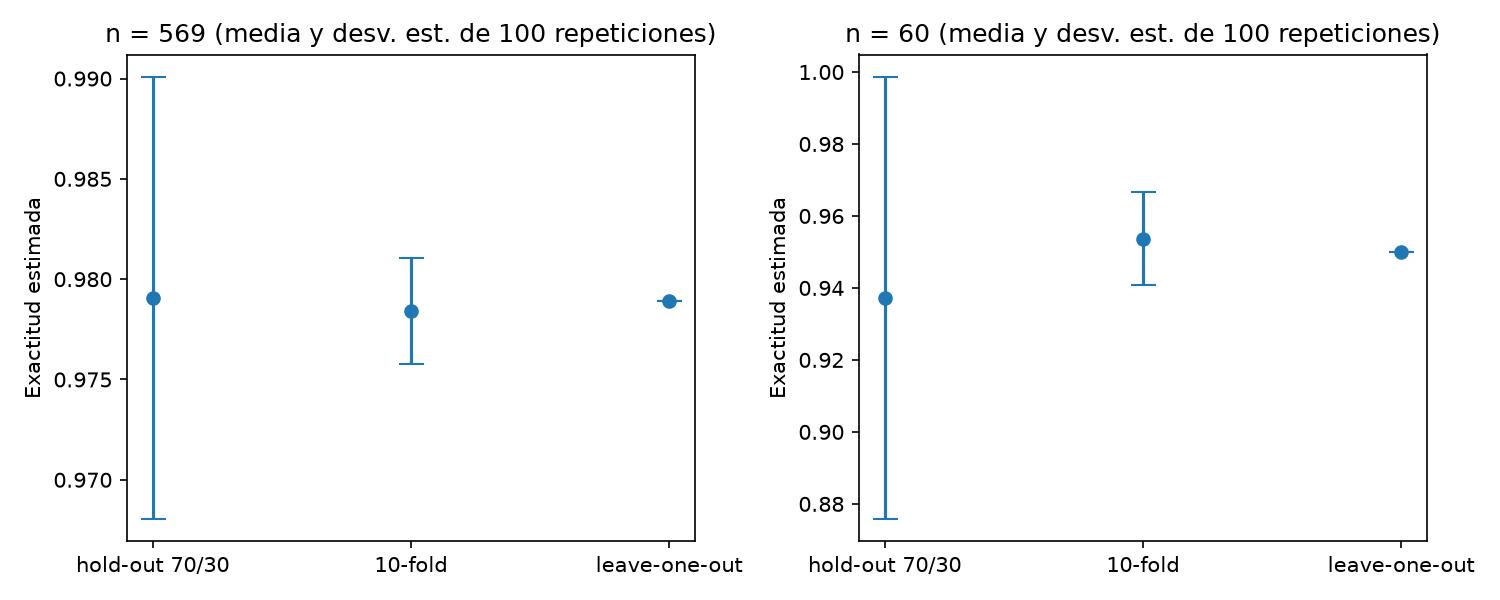
\includegraphics[width=\textwidth]{img/variabilidad_metodos.png}
\caption{Variación de la exactitud estimada con cada método de partición, con el conjunto completo y con una submuestra de 60 pacientes.}
\label{fig:var}
\end{figure}

Con 569 pacientes, la exactitud estimada por hold-out varía entre 0.9415 y 1.0000 según la partición (desviación estándar de 0.0110), la de 10-fold entre 0.9701 y 0.9842 (0.0026) y leave-one-out es determinista. Con solo 60 pacientes el hold-out se vuelve poco confiable: su desviación estándar es 0.0615 y va de 0.7778 a 1.0000, porque la prueba tiene 18 pacientes y cada error resta 5.6 puntos. La validación cruzada de 10 particiones se mantiene estable (0.0129) y su media (0.9537) queda cerca de la de leave-one-out (0.9500). Esto confirma el criterio del tema: hold-out cuando hay datos suficientes, y validación cruzada o leave-one-out cuando hay pocos \parencite{tecnm2026_tema33}.

\textbf{Método elegido.} Con 569 instancias hay datos suficientes para un hold-out, pero su estimación depende de la partición y estima la sensibilidad con muy pocos casos malignos. La validación cruzada de 10 particiones usa todos los datos para probar, es estable y cuesta 10 entrenamientos en lugar de 569, así que es el método más adecuado para este conjunto. Leave-one-out da un resultado equivalente, pero es más costoso y se justifica sobre todo con muy pocas instancias, como en los estudios genómicos. Con cualquiera de los dos hay que recordar que las observaciones no son independientes, así que sus resultados no deben usarse directamente con pruebas paramétricas \parencite{tecnm2026_tema33}.

\subsection{Tarea 2: Resultados de efectividad y métrica adecuada}

El Código~\ref{cod:t6} reúne las métricas de los tres métodos, dibuja las matrices de confusión (Figura~\ref{fig:matrices}) y genera el reporte automático.

\begin{codigo}[label=cod:t6]{Tarea 2: métricas y reporte automático}
print("\n=== Tarea 2: resultados de efectividad ===")
comparacion = pd.DataFrame({'hold-out 70/30': res_holdout, '10-fold': res_cv10,
                            'leave-one-out': res_loo}).T
comparacion.index.name = 'método'
comparacion[['VP', 'FN', 'FP', 'VN']] = comparacion[['VP', 'FN', 'FP', 'VN']].astype(int)
columnas = ['exactitud', 'precisión', 'sensibilidad', 'especificidad', 'F1',
            'exactitud balanceada', 'AUC-ROC']
print(comparacion[columnas].T.round(4).to_string())
print(f"\nCosto de los errores en leave-one-out: {res_loo['FN']} falsos negativos (malignos no detectados) y "
      f"{res_loo['FP']} falsos positivos (benignos señalados como malignos)")

# Matrices de confusión de los tres métodos
fig, ejes = plt.subplots(1, 3, figsize=(12, 3.8))
for eje, (nombre, r) in zip(ejes, comparacion.iterrows()):
    matriz = np.array([[r['VP'], r['FN']], [r['FP'], r['VN']]])
    eje.imshow(matriz, cmap='Blues')
    for i in range(2):
        for j in range(2):
            eje.text(j, i, int(matriz[i, j]), ha='center', va='center', fontsize=14,
                     color='white' if matriz[i, j] > matriz.max() / 2 else 'black')
    eje.set_xticks([0, 1], ['maligno', 'benigno'])
    eje.set_yticks([0, 1], ['maligno', 'benigno'])
    eje.set_xlabel('Predicción')
    eje.set_ylabel('Clase real')
    eje.set_title(nombre)
guardar('matrices_confusion.png')

# Reporte automático: tablas en CSV y resumen en Markdown dentro de resultados/
comparacion[['VP', 'FN', 'FP', 'VN'] + columnas].round(4).to_csv(os.path.join(CARPETA_RES, 'metricas_por_metodo.csv'))
variabilidad.round(4).to_csv(os.path.join(CARPETA_RES, 'variabilidad_metodos.csv'), index=False)
metrica_principal = 'sensibilidad'
with open(os.path.join(CARPETA_RES, 'reporte_automatico.md'), 'w', encoding='utf-8') as f:
    f.write("# Reporte automático: clasificación de Breast Cancer Wisconsin (Diagnostic)\n\n")
    f.write(f"- Instancias: {len(X)}; variables: {X.shape[1]}; clase positiva: maligno "
            f"({int(y.sum())} casos, {y.mean():.1%}).\n")
    f.write("- Clasificador: regresión logística con variables estandarizadas.\n")
    f.write(f"- Métrica principal: {metrica_principal} (un falso negativo es un cáncer no detectado).\n\n")
    f.write("## Métricas por método de partición\n\n")
    f.write(a_markdown(comparacion[['VP', 'FN', 'FP', 'VN'] + columnas].round(4)) + "\n\n")
    f.write("## Variabilidad de la exactitud según el método y el tamaño del conjunto\n\n")
    f.write(a_markdown(variabilidad.round(4), indice=False) + "\n")
print("\nReporte automático guardado en la carpeta resultados/")
print("Archivos:", sorted(os.listdir(CARPETA_RES)))
\end{codigo}

\begin{consola}[label=out:t6]{Ejecución de \texttt{act21.py}: Tarea 2}
=== Tarea 2: resultados de efectividad ===
método                hold-out 70/30  10-fold  leave-one-out
exactitud                     0.9708   0.9754         0.9789
precisión                     0.9836   0.9806         0.9762
sensibilidad                  0.9375   0.9528         0.9670
especificidad                 0.9907   0.9888         0.9860
F1                            0.9600   0.9665         0.9716
exactitud balanceada          0.9641   0.9708         0.9765
AUC-ROC                       0.9975   0.9947         0.9947

Costo de los errores en leave-one-out: 7 falsos negativos (malignos no detectados) y 5 falsos positivos (benignos señalados como malignos)

Reporte automático guardado en la carpeta resultados/
Archivos: ['metricas_por_metodo.csv', 'reporte_automatico.md', 'variabilidad_metodos.csv']
\end{consola}

\begin{figure}[htbp]
\centering
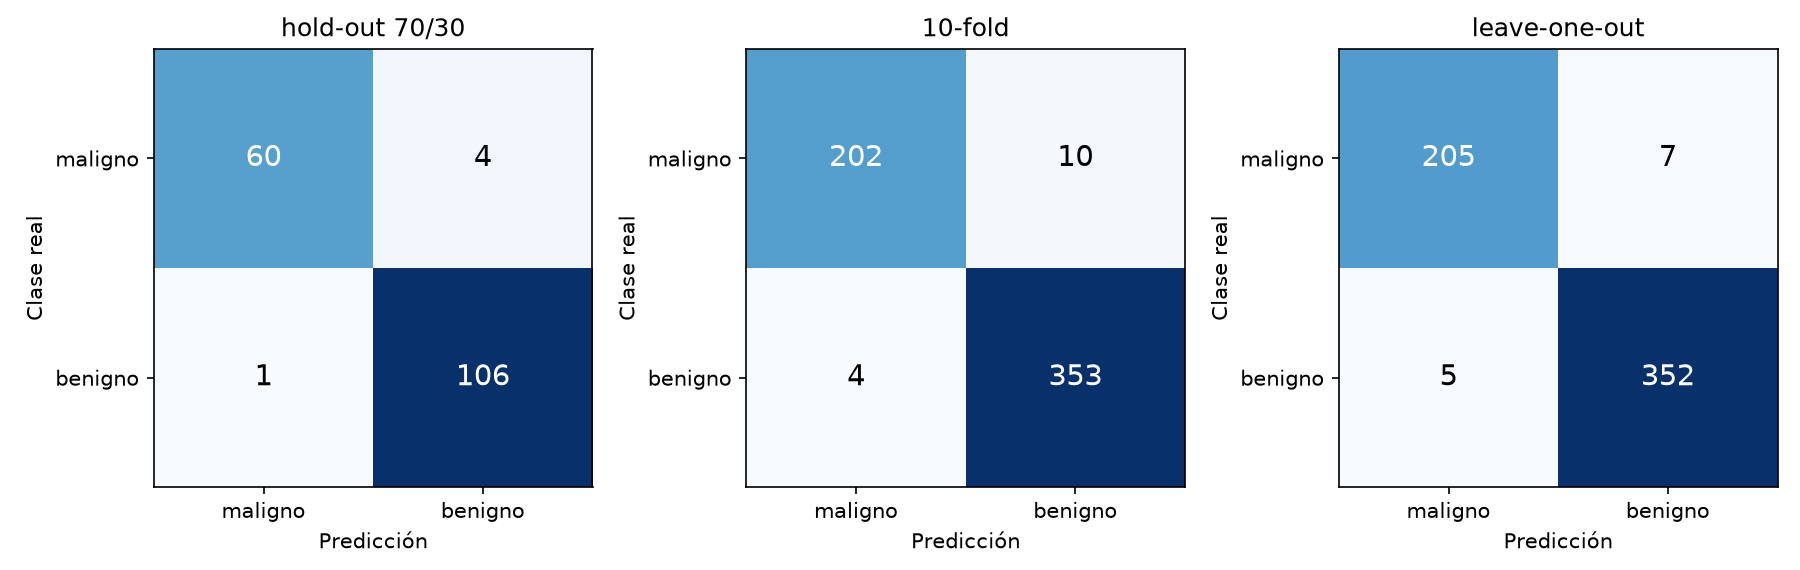
\includegraphics[width=\textwidth]{img/matrices_confusion.png}
\caption{Matrices de confusión de la regresión logística con cada método de partición (clase positiva: maligno).}
\label{fig:matrices}
\end{figure}

\textbf{Resultados.} Con el método elegido (10-fold), el clasificador alcanza una exactitud de 0.9754, una precisión de 0.9806, una sensibilidad de 0.9528, una especificidad de 0.9888, un $F_1$ de 0.9665 y un AUC-ROC de 0.9947. Es decir, detecta 202 de los 212 tumores malignos y señala por error como malignos a 4 de los 357 benignos. Con leave-one-out los valores son parecidos (sensibilidad 0.9670, 7 falsos negativos y 5 falsos positivos), y el AUC-ROC es casi idéntico (0.9947) en los tres métodos.

\textbf{Métrica más adecuada: la sensibilidad, acompañada de la especificidad y el AUC-ROC.} La razón está en la naturaleza del problema. Es un diagnóstico de enfermedad, donde el falso negativo (un cáncer que no se detecta) cuesta más que el falso positivo (una paciente sana que se somete a más estudios), porque a la enferma se le puede negar un tratamiento a tiempo \parencite{tecnm2026_tema33}. La sensibilidad es la métrica que mide justamente esos falsos negativos. La exactitud, en cambio, no es suficiente: el conjunto está desbalanceado (37.3\,\% de malignos), un modelo trivial alcanza 0.627 y, sobre todo, la exactitud trata igual los dos errores, y aquí tienen costos distintos. La especificidad vigila el otro error, el de los falsos positivos, y el AUC-ROC resume qué tan bien separa el modelo las dos clases con todos los umbrales posibles, sin favorecer a la clase mayoritaria \parencite{tecnm2026_tema33}. Con estos criterios, el resultado a reportar es una sensibilidad de 0.953 con una especificidad de 0.989.

\subsection{Reporte automático}

Al terminar, el script guarda en la carpeta \texttt{resultados/} el archivo \texttt{metricas\_por\_metodo.csv} (matriz de confusión y métricas de cada método), \texttt{variabilidad\_metodos.csv} (resultados de la Tarea 1d) y \texttt{reporte\_automatico.md}, un resumen con la descripción del conjunto, la métrica principal y las dos tablas. Las figuras de este reporte se generan en \texttt{img/}. Para analizar otro conjunto de datos solo hay que cambiar la sección de selección de datos; el resto del análisis y los archivos se generan igual.

\section{Conclusiones}

Con el conjunto Breast Cancer Wisconsin (569 pacientes, 37.3\,\% malignos), los tres métodos de partición dieron resultados parecidos para una regresión logística: exactitud entre 0.971 y 0.979 y sensibilidad entre 0.938 y 0.967. Las diferencias se explican por cómo se parte el conjunto, no por el modelo. El estudio de variabilidad mostró que el hold-out es el menos estable, sobre todo con pocos datos (desviación estándar de 0.062 con 60 pacientes contra 0.013 de la validación cruzada), y que la validación cruzada de 10 particiones es el mejor compromiso para este conjunto, con leave-one-out reservado para conjuntos muy pequeños.

En un problema de diagnóstico la métrica principal debe ser la sensibilidad, porque un falso negativo es un cáncer no detectado, complementada con la especificidad y el AUC-ROC; la exactitud sola es engañosa con clases desbalanceadas y con errores de costo distinto. El resultado final es una sensibilidad de 0.953 y una especificidad de 0.989 con validación cruzada de 10 particiones. Como en cualquier validación por partición, la estimación vale para este conjunto de datos y no garantiza el desempeño en otra población de pacientes.

\referencias

\end{document}
